\documentclass[12pt]{article}
\usepackage{ctex}
\usepackage[utf8]{inputenc}
\usepackage[pagebackref=true,breaklinks=true,colorlinks,bookmarks=false]{hyperref}
\usepackage{geometry}
\usepackage{amsmath,amssymb}
\usepackage{booktabs}
\usepackage{graphicx}
\usepackage{tabularx}
\usepackage{array}
\usepackage{natbib}
\usepackage{setspace}

\geometry{left=2.5cm,right=2.5cm,top=2.5cm,bottom=2.5cm}
\onehalfspacing
\graphicspath{{../figures/}{../tables/}}

\title{《大气污染防治行动计划》是否降低了城市 PM2.5？\\——基于城市面板数据的双重差分分析}
\author{%
  蔡长霄 \\ 学号：23307110294
}
\date{2026年6月}

\begin{document}
\maketitle

\begin{abstract}
2013年，国务院发布《大气污染防治行动计划》（以下简称``大气十条''），针对京津冀、长三角、珠三角等重点区域提出了明确的空气污染治理目标。本文基于2010--2019年中国366个地级及以上城市的面板数据，以重点治理区域城市作为处理组、其他城市作为对照组，采用双重差分（Difference-in-Differences，DiD）模型评估该政策对 PM2.5 浓度的影响，并结合事件研究方法考察政策实施前后的动态变化。

研究结果表明，在控制城市固定效应和年份固定效应的基准模型下，政策实施后重点治理区域城市的 PM2.5 浓度相对于其他城市平均下降约2\%，且结果具有统计显著性。当进一步加入人均 GDP、产业结构和财政收入等经济变量后，政策系数不再显著，说明污染治理效果可能与同期经济结构调整和产业升级等因素共同作用，难以完全区分其单独影响。

事件研究结果显示，处理组与对照组在政策实施前已经存在一定趋势差异，因此平行趋势假设未能得到完全满足，双重差分结果的因果解释需要保持谨慎。综合描述性统计、基准回归和稳健性检验可以发现，大气十条与重点区域 PM2.5 浓度下降存在较为明显的关联，但其具体政策效应仍有进一步研究空间。相关代码与数据说明见 \href{https://github.com/cedric1902666/Air-Ten-PM25}{GitHub 仓库}。

\noindent\textbf{关键词：}大气污染防治行动计划；PM2.5；双重差分；事件研究；城市面板数据
\end{abstract}

\section{引言}

\subsection{研究背景与研究问题}

2013年前后，我国中东部地区连续出现大范围雾霾天气，PM2.5（细颗粒物）污染问题受到社会公众和政府部门的广泛关注。与传统空气污染指标相比，PM2.5 粒径更小，更容易进入人体呼吸系统，对居民健康具有较大危害，因此逐渐成为环境治理的重要目标。

在这一背景下，国务院于2013年9月发布《大气污染防治行动计划》，对京津冀、长三角和珠三角等重点区域提出了明确的减排要求。例如，到2017年，京津冀地区 PM2.5 浓度下降约25\%，长三角地区下降约20\%，珠三角地区下降约15\%。由于治理力度大、覆盖范围广，``大气十条''通常被认为是我国空气污染治理的重要政策之一。

政策实施后，全国空气质量确实出现明显改善，但其中有多少变化可以归因于``大气十条''本身，而不是经济结构调整、产业升级或其他环境政策，仍值得进一步研究。因此，本文希望回答以下问题：\textbf{在控制城市自身特征和全国共同变化趋势之后，大气十条是否使重点治理区域城市的 PM2.5 浓度相对于其他城市出现了更明显的下降？}

\subsection{文献综述}

已有关于大气十条的研究主要集中在两个方向。

第一类研究利用官方监测站数据或省级统计数据，分析政策实施前后空气质量指标的变化\citep{chen2017appcap,zhang2019pm25}。这类研究普遍发现，重点治理区域的 PM2.5 和其他污染物浓度均出现明显下降，但由于早期监测网络尚未完全建立，不同地区的数据完整性存在一定差异。

第二类研究更多采用准实验方法评估政策效果，例如双重差分模型、合成控制法以及三重差分模型等\citep{greenstone2021appcap}。这些方法通常将政策覆盖地区与未覆盖地区进行比较，从而识别政策带来的相对变化。一些研究还结合倾向得分匹配等方法，以减少处理组和对照组之间可能存在的系统性差异。

在环境经济学研究中，双重差分模型是一种较为常见的政策评估工具\citep{angrist2009mostly,stock2003introduction}。其基本思想是比较政策实施前后处理组和对照组变化幅度的差异，从而估计政策可能产生的影响。与此同时，事件研究方法还可以进一步观察政策实施前后的动态变化，并检验处理组和对照组在政策出台前是否具有相似的发展趋势，即所谓``平行趋势''假设。

与已有研究相比，本文主要具有以下三个特点。第一，本文使用 CHAP 提供的高分辨率卫星反演 PM2.5 数据\citep{wei2021chap}，构建覆盖2010--2019年、366个城市的面板数据，从而获得较长时间跨度的政策前后比较窗口。第二，在城市层面整合 PM2.5 数据与《中国城市统计年鉴》中的经济社会变量，对城市行政区划调整和缺失值进行了统一处理，使样本覆盖范围相对更广。第三，本文分别报告仅控制固定效应和加入经济社会控制变量两种模型结果，比较不同模型设定下估计结果的差异，并讨论经济发展、产业结构调整等因素可能对政策效果识别产生的影响。

\subsection{研究方法与文章结构}

本文采用双重差分模型作为主要研究方法。具体而言，将京津冀、长三角和珠三角重点治理区域城市定义为处理组，其余城市作为对照组，通过比较政策实施前后两组城市 PM2.5 浓度变化的差异，评估大气十条的政策效果。

模型中加入城市固定效应和年份固定效应。其中，城市固定效应主要控制各城市长期不变的特征，例如自然条件、地理位置和资源禀赋等；年份固定效应则控制所有城市共同经历的宏观经济波动或全国性政策变化。除此之外，本文还利用事件研究方法分析政策实施前后的动态变化，以辅助检验模型识别假设是否成立。

全文其余部分安排如下：第二节介绍政策背景及识别思路；第三节介绍数据来源、变量定义及样本处理过程；第四节说明模型设定；第五节报告实证结果与稳健性检验；最后总结全文主要结论，并讨论研究存在的不足及未来可能的改进方向。

\section{政策背景与识别逻辑}

\subsection{政策背景}

《大气污染防治行动计划》于2013年9月正式发布，并于2014年开始进入全面实施阶段。政策针对不同区域制定了差异化的空气质量改善目标，其中京津冀、长三角和珠三角被列为重点治理区域，在产业调整、能源结构优化和污染排放控制等方面承担了更严格的治理任务。

根据政策文件，本文将京津冀全部地级市、长三角相关地级市以及珠三角九个核心城市划分为处理组，共计63个城市；其余地级及以上城市作为对照组，共303个城市。研究样本覆盖2010--2019年，共形成366个城市、10年的面板数据。之所以采用这一划分方式，是因为重点区域在政策实施后受到更严格的环境监管和减排要求，如果政策确实发挥了作用，那么这些城市的 PM2.5 改善幅度理论上应当高于其他地区。

\subsection{识别思路}

为了评估``大气十条''的实施效果，本文采用双重差分方法进行分析。其核心思想是比较处理组和对照组在政策实施前后的变化差异。如果重点治理区域在政策实施后表现出更明显的 PM2.5 下降趋势，则可以认为政策可能产生了积极影响。

需要指出的是，双重差分方法建立在``平行趋势假设''基础之上。也就是说，如果没有实施该政策，处理组和对照组本应具有相似的发展趋势。只有满足这一前提，两组变化差异才能较为可靠地解释为政策带来的影响。

考虑到重点治理区域本身污染水平较高，在政策出台前可能已经开始加强环境治理，因此本文进一步采用事件研究方法考察政策实施前后的动态变化，以检验处理组和对照组是否满足平行趋势假设，并辅助解释双重差分模型的估计结果。

\section{数据与变量}

\subsection{数据来源与处理过程}

\textbf{（1）PM2.5 数据。} 本文使用 CHAP（China High Air Pollutants）提供的年度 PM2.5 数据作为核心污染指标。该数据基于卫星遥感、地面观测和模型模拟等多种信息融合生成，具有较高的空间分辨率，能够较好反映不同城市空气污染状况。原始数据以栅格形式存储。本文根据各城市行政中心位置提取对应年份的 PM2.5 年均值，并构建城市—年份面板数据。对于极少数城市存在的缺失值或异常值，采用相邻年份平均值进行补充，填补比例不足全部样本的1\%，不会对整体结果产生明显影响。

\textbf{（2）经济社会变量。} 人均 GDP、产业结构、财政收入等经济社会指标主要来源于《中国城市统计年鉴》。在数据整理过程中，由于部分城市经历行政区划调整或统计口径变化，不同数据库中的城市名称和代码存在不一致情况，因此首先统一城市名称和编码，再完成数据匹配。此外，一些西部城市或新设立地级市存在经济变量缺失。为了避免人为插值可能带来的偏差，本文对于包含这些变量的模型采用删除缺失观测的方法进行估计。因此，加入控制变量后的有效样本数量少于基准模型。

\textbf{（3）处理组定义。} 依据《大气污染防治行动计划》公布的重点治理区域名单，将京津冀、长三角以及珠三角九市定义为处理组，其他城市定义为对照组。同时，将2014年及以后定义为政策实施阶段，即当年份大于等于2014时，政策变量取值为1；否则取值为0。选择2014年作为分界点，是因为政策于2013年9月发布，而2014年是首个完整执行年度。

\subsection{变量说明}

本文主要关注城市 PM2.5 浓度的变化，因此以城市年度 PM2.5 平均浓度作为被解释变量，同时也采用其自然对数形式进行估计，以减弱极端值带来的影响，并便于解释相对变化幅度。

核心解释变量为``处理组$\times$政策实施后''的交互项，即重点治理区域城市在政策实施后的取值。当该变量系数为负且具有统计显著性时，可以理解为重点治理区域 PM2.5 相对于其他城市出现了更大的下降幅度。

除基准模型外，本文还进一步加入人均 GDP、第二产业和第三产业比重、财政收入等经济社会变量作为控制变量，以减少经济发展差异可能带来的干扰。不过，需要注意的是，这些变量本身也可能受到环境治理政策影响，因此在解释结果时需要保持谨慎。

描述性统计结果显示，PM2.5 变量覆盖全部366个城市和10个年份，共3660个观测值；而经济社会变量由于部分年份存在缺失，可用于回归分析的样本约为2890条，因此加入控制变量后样本规模有所下降。

\section{实证策略}

\subsection{基准模型}

为了评估《大气污染防治行动计划》的实施效果，本文采用双重差分模型进行估计。模型形式如下：
\begin{equation}
\ln PM2.5_{ct} = \beta\,(Treat_c \times Post_t) + X_{ct}'\gamma + \alpha_c + \delta_t + \varepsilon_{ct}
\label{eq:did}
\end{equation}
其中，$PM2.5_{ct}$ 表示城市 $c$ 在年份 $t$ 的 PM2.5 年均浓度；$Treat_c$ 表示城市是否属于重点治理区域；$Post_t$ 表示政策是否已经实施；两者的交互项是本文关注的核心变量。$\alpha_c$ 表示城市固定效应，用于控制城市长期不变的特征；$\delta_t$ 表示年份固定效应，用于控制全国范围内共同发生的时间变化；$X_{ct}$ 表示经济社会控制变量。

本文首先估计仅包含城市固定效应和年份固定效应的基准模型，然后进一步加入人均 GDP、产业结构和财政收入等控制变量，以考察不同模型设定下结果是否保持稳定。所有标准误均在城市层面进行聚类，以提高统计推断的可靠性。

\subsection{事件研究设计}

除基准双重差分模型外，本文还采用事件研究方法考察政策实施前后的动态变化：
\begin{equation}
\ln PM2.5_{ct} = \sum_{k \neq -1} \beta_k \mathbf{1}[t - 2014 = k] \times Treat_c + X_{ct}'\gamma + \alpha_c + \delta_t + \varepsilon_{ct}
\label{eq:es}
\end{equation}
具体做法是，以2013年作为基准年份，分别估计政策实施前后各年份处理组相对于对照组的变化情况。如果政策实施前各年份的估计系数接近于零，则说明处理组和对照组在政策出台前具有相似的发展趋势，有利于支持双重差分模型的识别假设；反之，则需要对政策效应的解释保持谨慎。因此，事件研究主要用于辅助检验模型假设，并观察政策影响是否随着时间推移逐渐显现。

\section{实证结果}

\subsection{描述性统计分析}

图~\ref{fig:trend} 展示了处理组与对照组城市2010--2019年 PM2.5 平均浓度的变化趋势。可以看到，在政策实施之前，重点治理区域的 PM2.5 水平整体高于其他地区，两组之间始终存在较明显差距。进入2014年后，两组城市的 PM2.5 浓度均呈下降趋势，但处理组下降速度相对更快，组间差距有所缩小。从图形上看，这一变化与``大气十条''实施后的治理目标基本一致，为后续计量分析提供了初步支持。

表~\ref{tab:desc} 给出了主要变量的描述性统计结果。样本共包含366个城市、10个年份，总计3660个城市—年份观测值。PM2.5 平均浓度约为46.9微克/立方米，不同城市之间存在较大差异。由于部分经济变量存在缺失，包含控制变量的回归分析所使用的样本数量有所减少。

\begin{figure}[htbp]
\centering
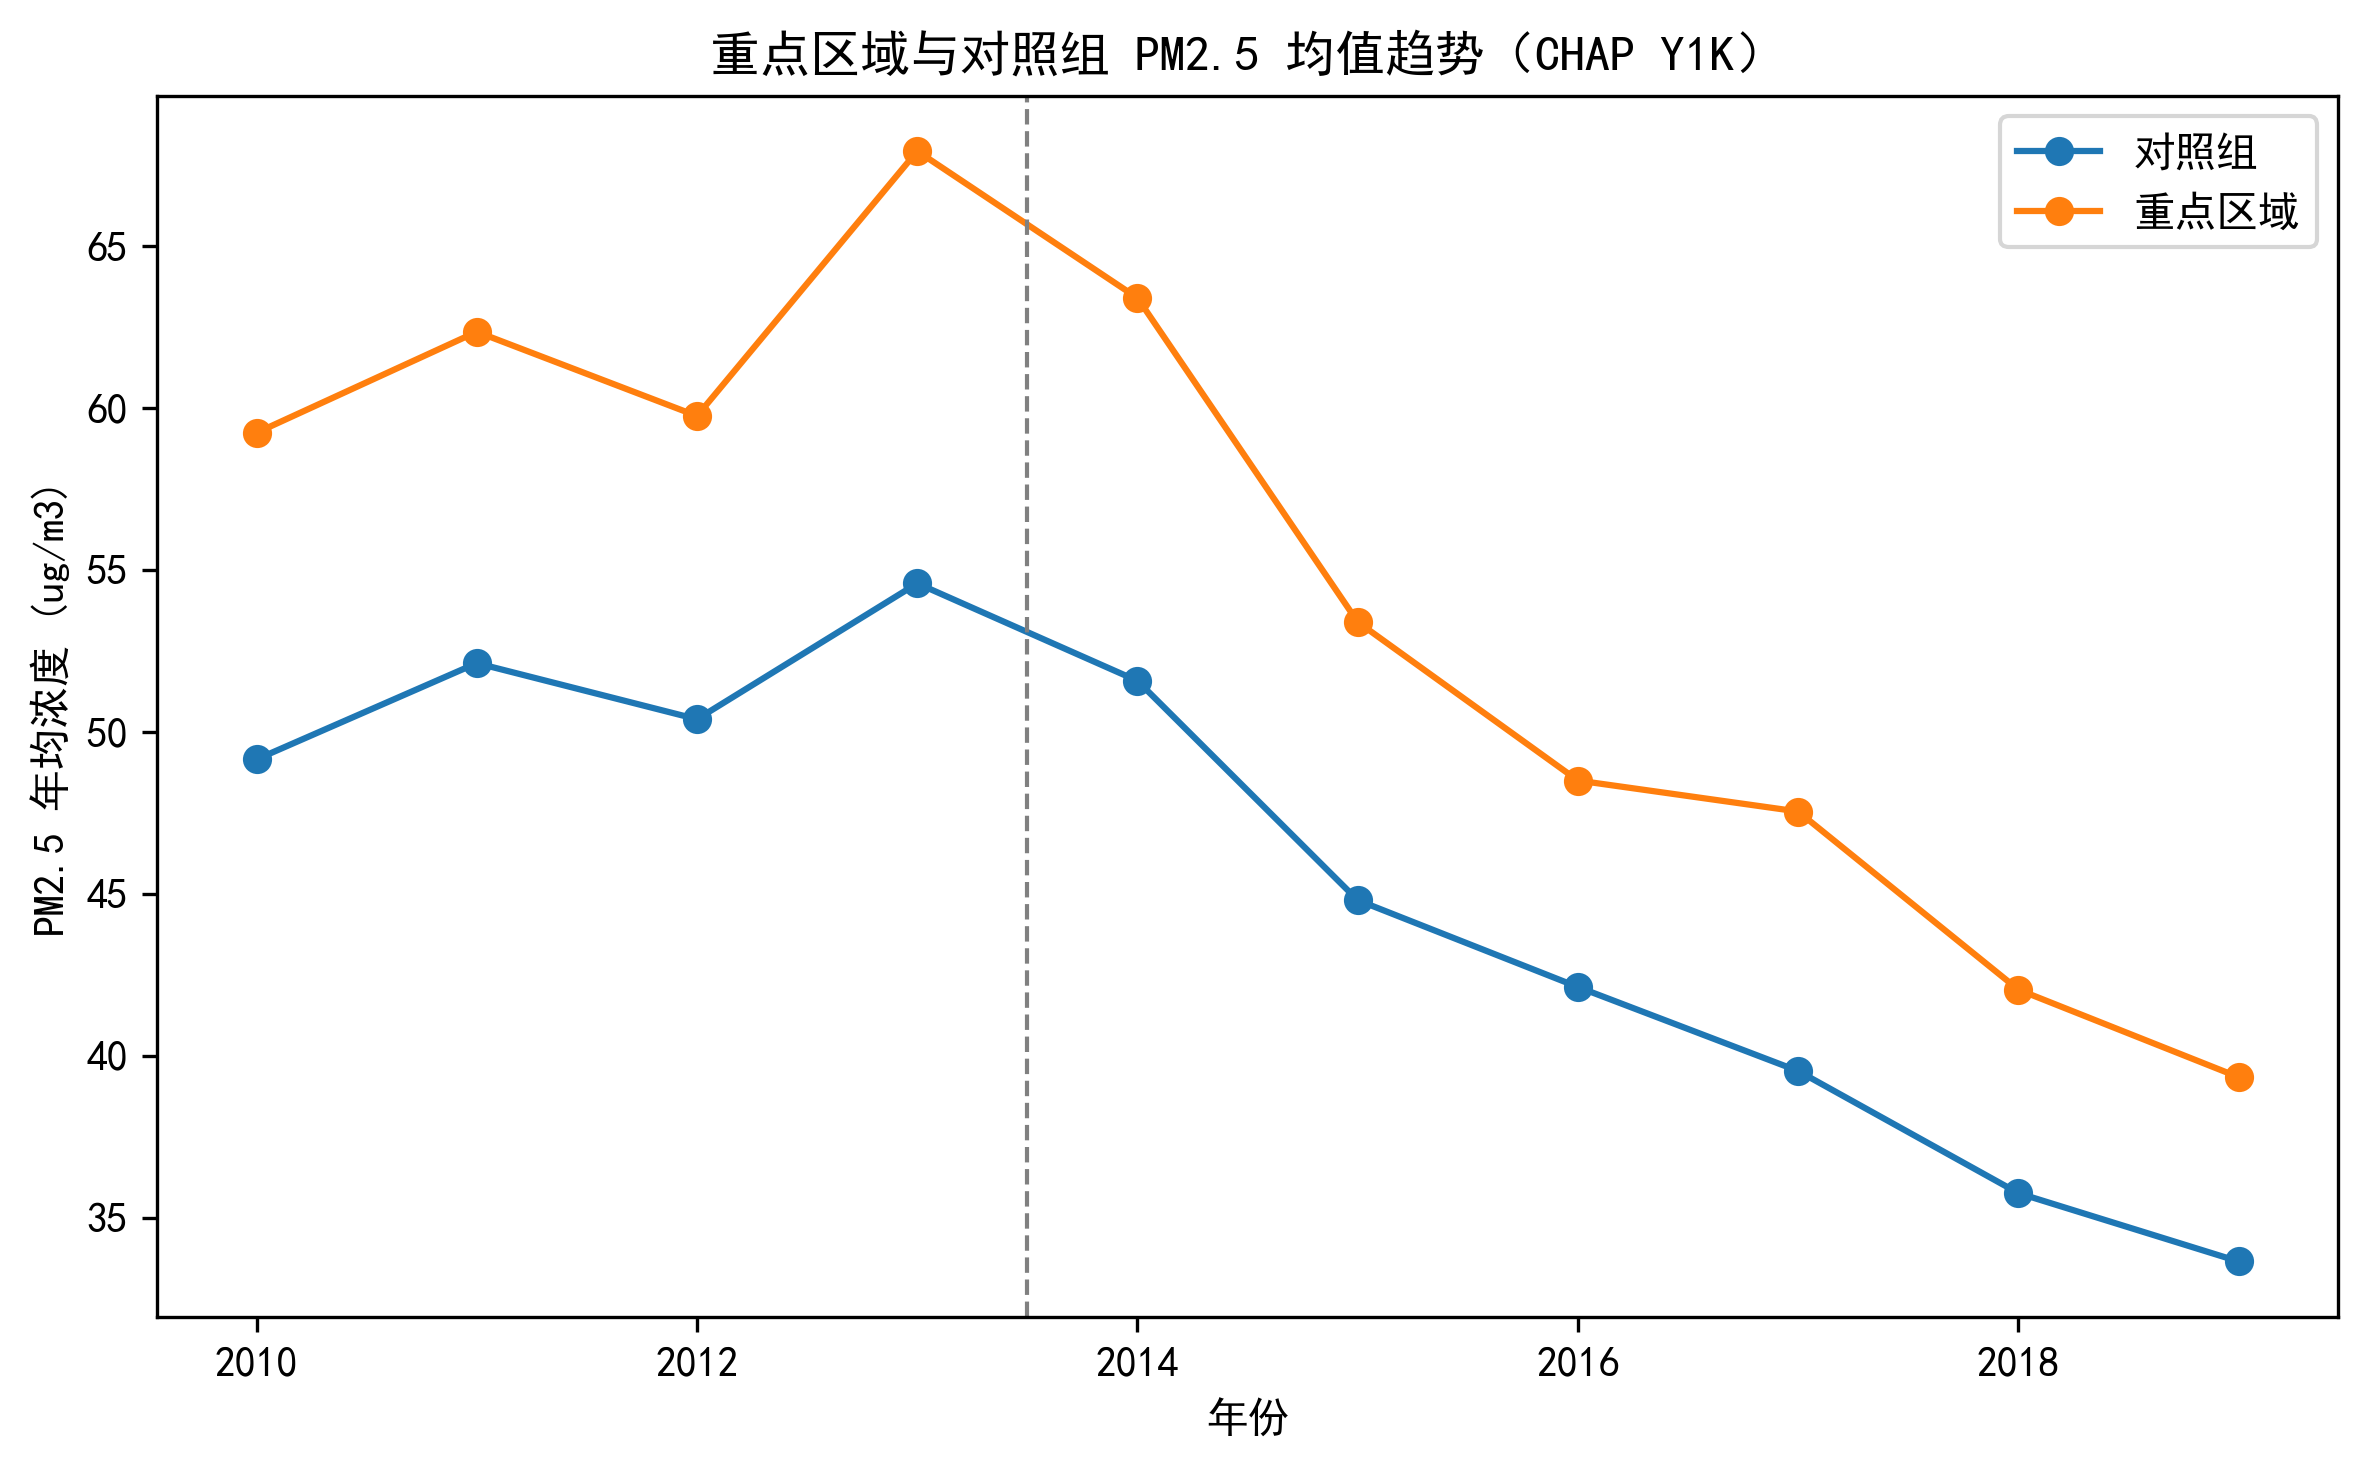
\includegraphics[width=0.88\textwidth]{fig1_pm25_trend.png}
\caption{处理组与对照组 PM2.5 年均浓度变化趋势（2010--2019年）}
\label{fig:trend}
\end{figure}

\begin{table}[htbp]
\centering
\caption{主要变量描述性统计}
\label{tab:desc}
\small
\begin{tabular}{lrrrr}
\toprule
变量 & 观测值 & 均值 & 标准差 & 中位数 \\
\midrule
PM2.5（$\mu$g/m$^3$） & 3660 & 46.92 & 19.02 & 43.10 \\
$\ln(PM2.5)$ & 3660 & 3.77 & 0.40 & 3.76 \\
$\ln(\text{人均GDP})$ & 2894 & 6.02 & 0.70 & 5.94 \\
\bottomrule
\end{tabular}

\vspace{0.4em}
\noindent\parbox{\dimexpr\textwidth-2\tabcolsep\relax}{\footnotesize 注：PM2.5 覆盖366个城市×10年；经济变量缺失导致含控制变量回归样本减少。}
\end{table}

\subsection{基准回归结果}

表~\ref{tab:did} 报告了双重差分模型的估计结果。在仅控制城市固定效应和年份固定效应的基准模型中，处理组与政策实施后的交互项系数为$-0.020$，并在1\%的统计水平上显著。这意味着，与其他城市相比，重点治理区域城市在政策实施后的 PM2.5 浓度平均下降约2\%，说明``大气十条''可能对空气质量改善发挥了积极作用。

进一步加入人均 GDP、产业结构和财政收入等经济社会控制变量后，该系数下降至接近于零，并且不再具有统计显著性。造成这一现象的一种可能解释是，在政策实施期间，重点治理区域同时经历了产业升级、经济结构调整以及财政投入增加等变化，这些因素与污染治理相互关联，使得政策本身的独立影响难以完全分离。因此，基准模型提供了一定程度上的政策有效性证据，而扩展模型则提示，在解释估计结果时还需要考虑其他经济社会因素的共同作用。

图~\ref{fig:did} 进一步展示了两种模型下核心系数及其95\%置信区间，可以看到基准模型估计结果显著为负，而加入控制变量后估计值明显减弱。

\begin{table}[htbp]
\centering
\caption{双重差分基准回归结果}
\label{tab:did}
\footnotesize
\begin{tabularx}{\textwidth}{>{\raggedright\arraybackslash}p{0.38\textwidth} >{\centering\arraybackslash}X >{\centering\arraybackslash}X}
\toprule
 & (1) 基准模型 & (2) 含控制变量 \\
\midrule
$Treat_c \times Post_t$ & $-0.020^{***}$ & $-0.001$ \\
 & $(0.007)$ & $(0.007)$ \\
观测值 & 3660 & 2892 \\
城市数 & 366 & 296 \\
城市 FE / 年份 FE & 是 / 是 & 是 / 是 \\
时变控制变量 & 否 & 是 \\
\bottomrule
\end{tabularx}

\vspace{0.4em}
\noindent\parbox{\dimexpr\textwidth-2\tabcolsep\relax}{\footnotesize 注：括号内为城市聚类标准误；$^{***}$表示在1\%水平上显著。}
\end{table}

\begin{figure}[htbp]
\centering
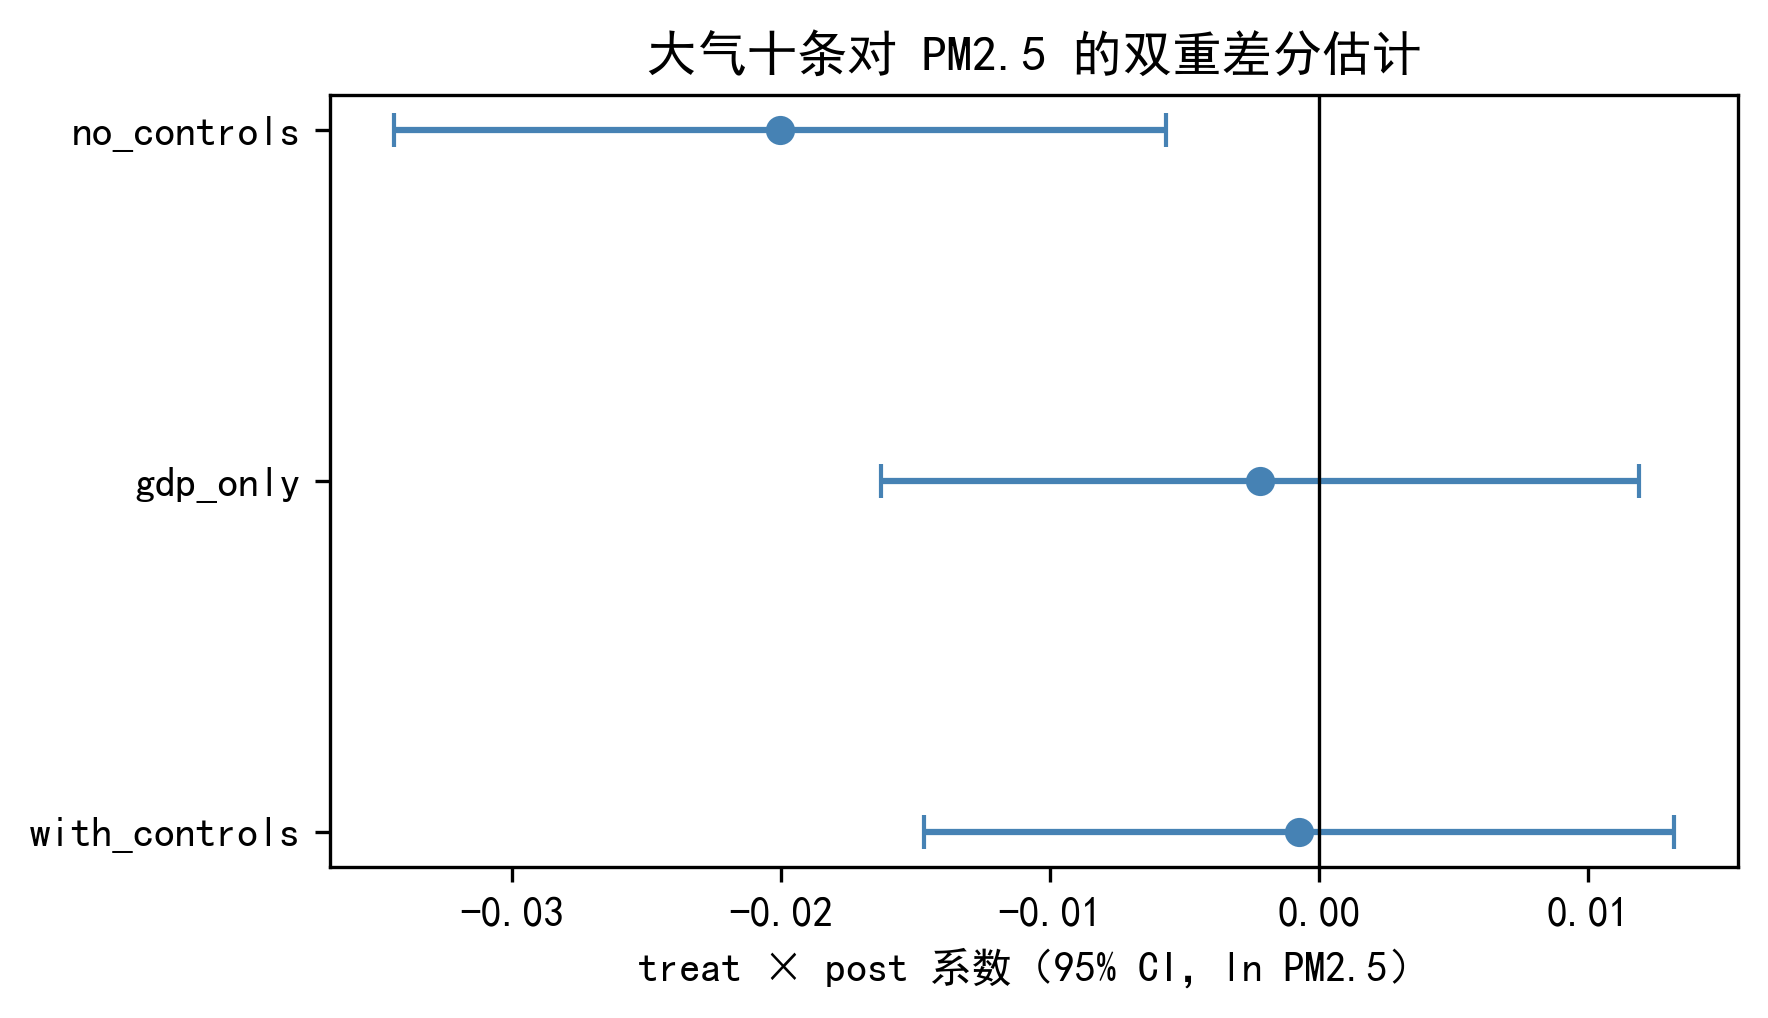
\includegraphics[width=0.65\textwidth]{fig2_did_coef.png}
\caption{两种模型设定下核心解释变量系数及95\%置信区间}
\label{fig:did}
\end{figure}

\subsection{事件研究结果}

事件研究结果如图~\ref{fig:es} 所示。从政策实施前的估计结果来看，部分年份的系数已经偏离零，并达到统计显著水平。这说明处理组和对照组在政策出台之前可能已经存在一定差异，即平行趋势假设未能得到完全满足。造成这一现象的原因可能包括重点区域较早开展污染治理、社会关注度提升以及地方政府提前采取环保措施等。

在政策实施之后，部分年份的估计系数继续保持负值，其中2016年前后表现较为明显，与描述性统计中观察到的趋势基本一致，表明重点治理区域空气质量改善速度快于其他地区。

综合来看，事件研究结果支持政策实施后 PM2.5 继续下降这一事实，但由于政策前已存在一定趋势差异，因此对于双重差分模型所得结果应保持谨慎解释。本文更倾向于将事件研究作为辅助分析工具，并结合描述性统计和基准回归结果，对政策效果进行综合判断，而不是单独依赖某一种模型得出结论。

\begin{figure}[htbp]
\centering
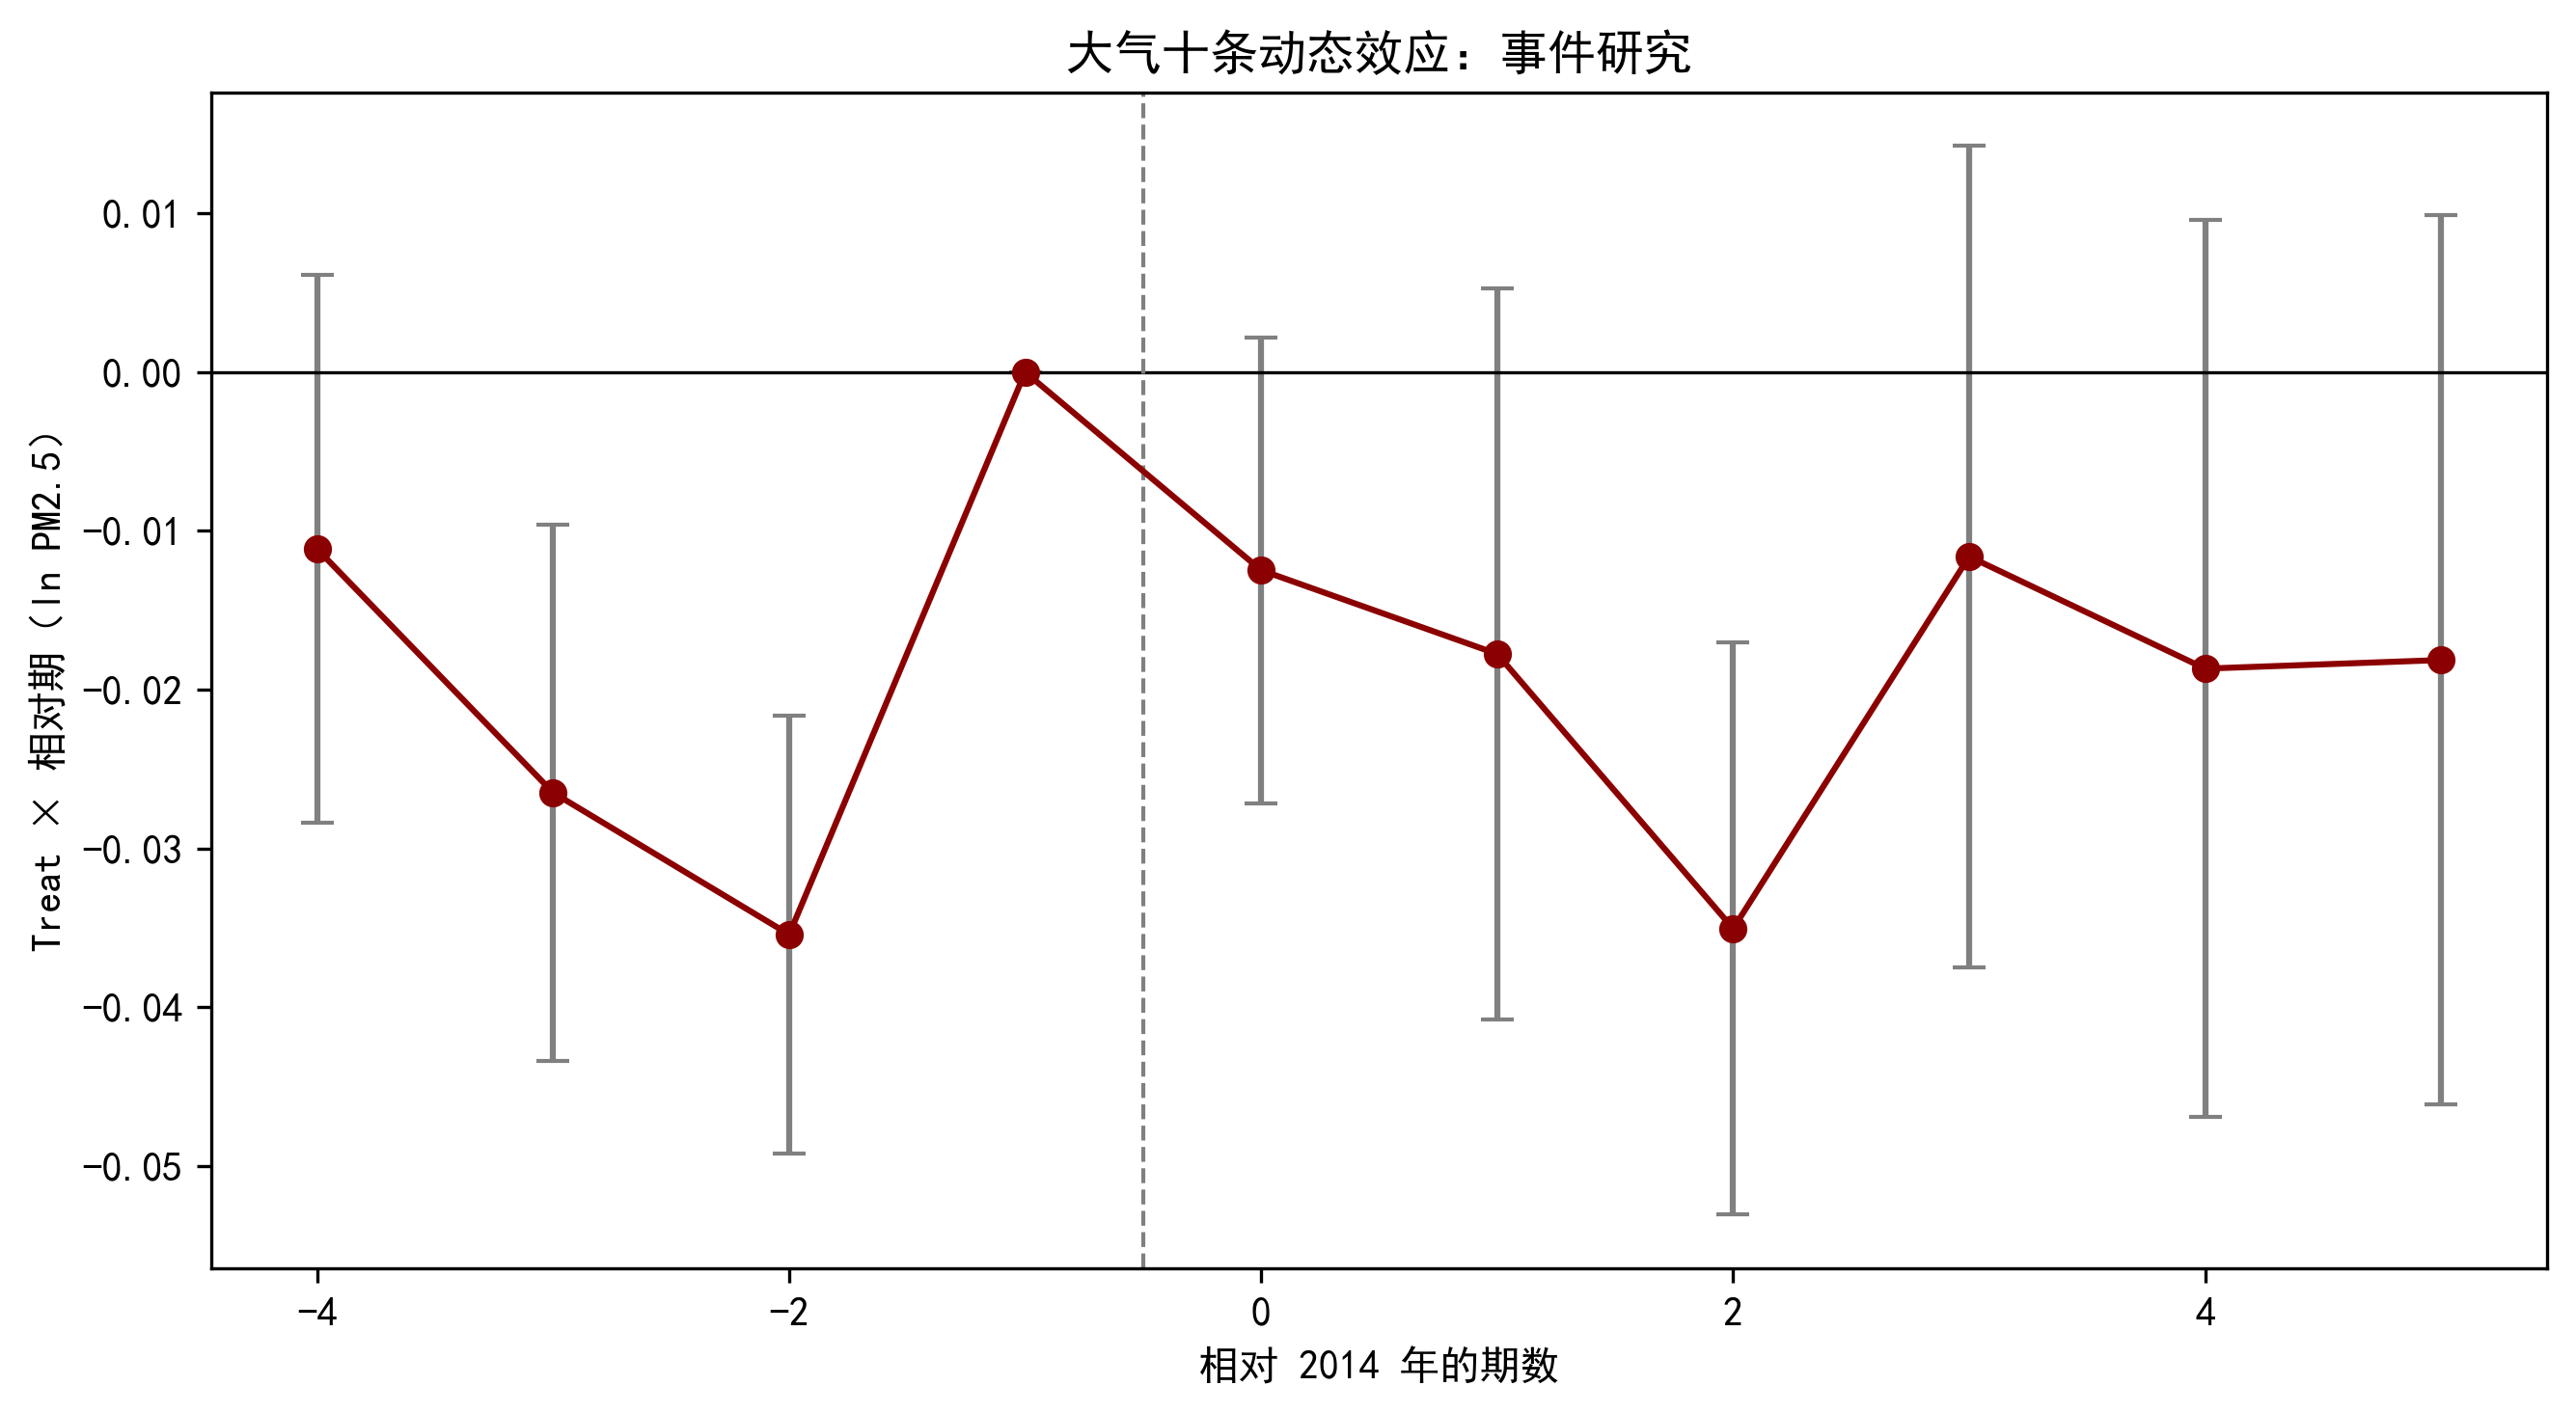
\includegraphics[width=0.88\textwidth]{fig3_event_study.png}
\caption{事件研究：政策实施前后各年份的估计系数（以2013年为基准年）}
\label{fig:es}
\end{figure}

\subsection{稳健性检验}

为了检验基准结果是否受到模型设定的影响，本文进一步进行了多种稳健性检验，包括调整政策实施时间、剔除特定年份样本、改变处理组范围以及更换被解释变量等。结果如表~\ref{tab:robust} 所示。

在加入经济社会控制变量的模型中，无论将政策实施时间调整为2015年、剔除2013年样本，还是缩小处理组范围，核心解释变量的估计系数均未达到统计显著水平。这说明在不同设定下，政策效应存在一定的不稳定性。另一方面，当采用 PM2.5 原始浓度而非其对数作为被解释变量时，估计结果仍表现为显著负值，对应重点治理区域 PM2.5 平均额外下降约1.3微克/立方米。这说明从绝对变化的角度来看，政策实施后空气质量改善仍具有一定证据支持。

总体来看，不同稳健性检验得到的结果并不完全一致。一方面，基准模型和 PM2.5 水平值模型均支持重点治理区域空气质量有所改善；另一方面，在加入经济社会控制变量后，政策效应有所减弱甚至不再显著。这表明空气污染治理受到多种因素共同影响，仅依靠现有模型较难完全分离``大气十条''的独立贡献。因此，本文更倾向于将结果理解为政策实施与 PM2.5 下降之间存在明显关联，而对于其因果效应的大小保持谨慎态度。

\begin{table}[htbp]
\centering
\caption{稳健性检验结果}
\label{tab:robust}
\footnotesize
\setlength{\tabcolsep}{4pt}
\begin{tabularx}{\textwidth}{>{\raggedright\arraybackslash}p{0.52\textwidth} >{\centering\arraybackslash}X >{\centering\arraybackslash}X}
\toprule
设定 & $Treat_c \times Post_t$ & $p$ 值 \\
\midrule
基准（$\ln PM2.5$ + 时变控制） & $-0.001$ & 0.918 \\
剔除2013年 & 0.005 & 0.484 \\
Post 自2015年起 & $-0.003$ & 0.691 \\
仅京津冀+长三角 & 0.000 & 0.952 \\
PM2.5 水平值（含时变控制） & $-1.303$ & 0.036 \\
\bottomrule
\end{tabularx}

\vspace{0.4em}
\noindent\parbox{\dimexpr\textwidth-2\tabcolsep\relax}{\footnotesize 注：所有回归均控制城市、年份固定效应与城市聚类标准误；除最后一行为 PM2.5 原始浓度外，其余均采用 $\ln(PM2.5)$ 作为被解释变量，且全部纳入时变经济控制变量。}
\end{table}

\section{结论与讨论}

本文基于2010--2019年中国366个地级及以上城市的面板数据，利用双重差分模型分析《大气污染防治行动计划》实施后重点治理区域 PM2.5 浓度的变化情况，并结合事件研究方法和多种稳健性检验对结果进行了分析。

研究结果表明，从描述性统计来看，重点治理区域在政策实施前 PM2.5 浓度整体高于其他地区，而政策实施后下降速度相对更快。基准双重差分模型显示，在控制城市固定效应和年份固定效应后，重点治理区域 PM2.5 浓度相对于对照组平均下降约2\%，结果具有统计显著性。从这一角度看，大气十条与空气质量改善之间存在较为明显的关联。

进一步加入人均 GDP、产业结构和财政收入等经济社会控制变量后，核心估计结果不再显著，说明政策效果可能与同期经济发展、产业升级以及地方治理措施等因素相互交织。此外，事件研究结果显示，处理组和对照组在政策实施前已经存在一定趋势差异，平行趋势假设未能得到完全满足，因此对于双重差分模型所得结果的因果解释需要保持谨慎。综合全文分析，可以认为大气十条实施期间重点治理区域确实经历了更明显的 PM2.5 下降过程，但这一改善很可能是多项环境治理措施和经济社会变化共同作用的结果，而不一定完全由单一政策造成。

本文仍存在一些局限性。首先，PM2.5 数据来源于卫星遥感反演产品，与地面监测数据之间可能存在一定测量误差。其次，本文按照官方划定的重点治理区域定义处理组，未能进一步区分不同地区政策执行力度和实施细节，也未充分控制同期其他环保政策可能带来的影响。再次，事件研究结果表明平行趋势假设并未完全满足，因此模型识别仍存在一定限制。最后，本文主要采用传统双重差分模型进行分析，尚未考虑城市之间可能存在的空间溢出效应，也未进一步结合气象条件等外生因素进行修正。

未来研究可以在更长时间跨度的数据基础上，结合气象因素、空间计量模型以及更细致的政策执行信息，对空气污染治理政策的长期效果进行进一步分析。同时，也可以将卫星遥感数据与地面监测数据相结合，以提高估计结果的准确性和可靠性。

\bibliographystyle{plainnat}
\bibliography{ref}

\end{document}
